\subsection*{หน้าต่าง Select}
\begin{figure}[!ht]
  \centering
    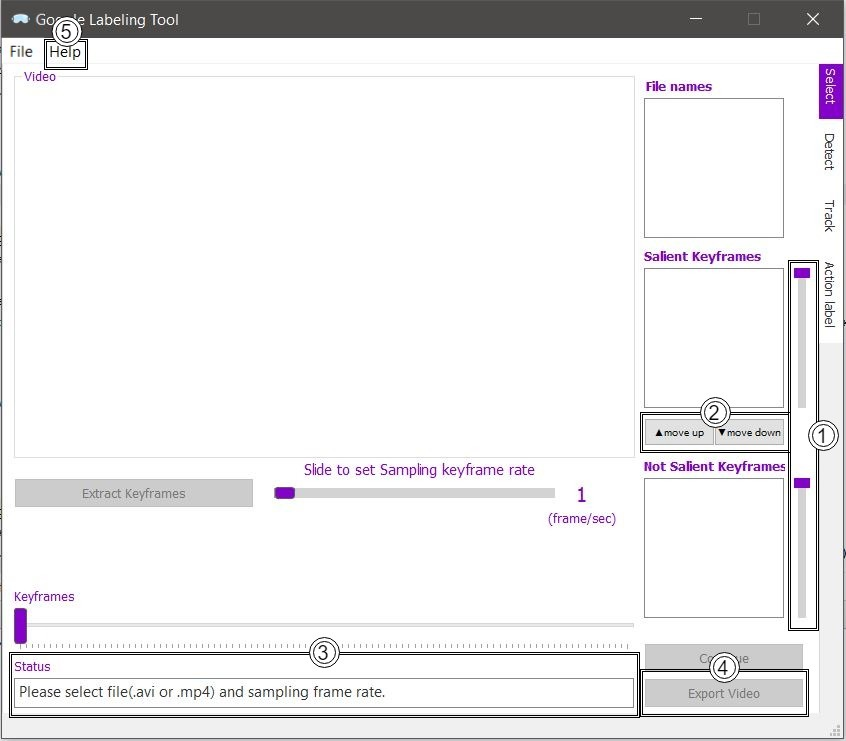
\includegraphics[scale=0.4]{chapter4/images/Final_ui/Select.jpg}
    \caption{รูปหน้าต่างแสดงผลของหน้าต่าง Select}
    \label{fig:final_select}
\end{figure}
จากรูปที่ \ref{fig:final_select} แสดงหน้าต่าง Select ของแอพพลิเคชั่น ซึ่งเมื่อเทียบกันกับฉบับร่างตามรูปที่ \ref{fig:SelectDraft} จะมีส่วนที่เพิ่มเติมขึ้นมาดังนี้
\begin{enumerate}
	\item แถบเลื่อนสำหรับเลื่อนดูเฟรมที่มีมนุษย์หรือไม่มีมนุษย์ เพื่อเพิ่มความสะดวกในการเลือกดูเฟรม
	\item ปุ่มสำหรับแก้ไขเฟรมที่มีมนุษย์หรือไม่มีมนุษย์
	\item แถบแสดงสถานะกระบวนการทำงาน
	\item ปุ่มสำหรับนำผลลัพธ์ออกเป็นไฟล์วิดิโอเฉพาะในช่วงที่มีมนุษย์อยู่
	\item แถบสำหรับคำแนะนำช่วยเหลือ
	\item ปุ่มสำหรับเปิดไฟล์
\end{enumerate}		

\clearpage
\subsection*{หน้าต่าง Detect}
\begin{figure}[!ht]
  \centering
    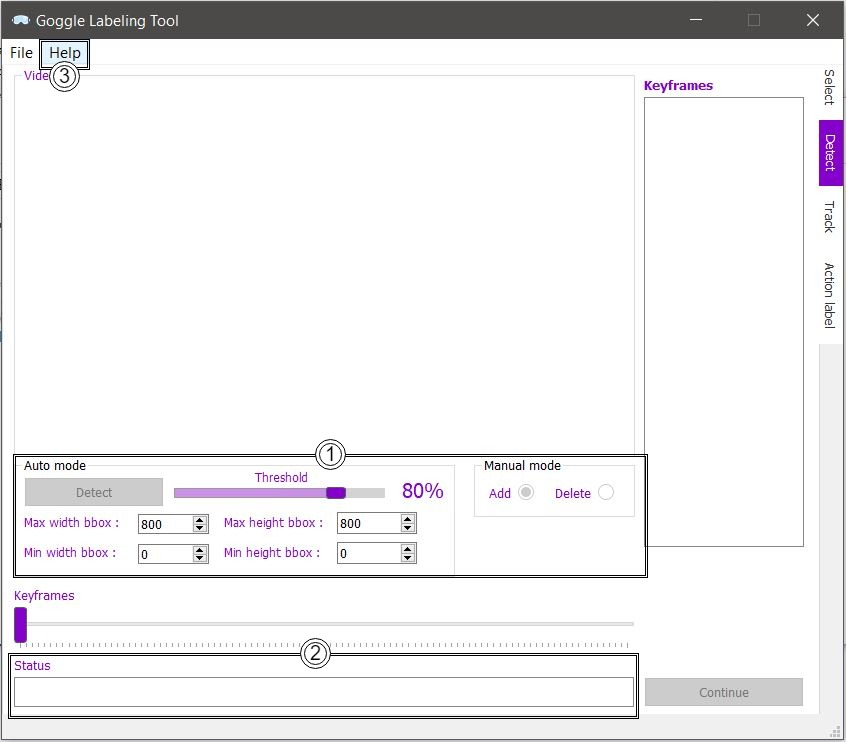
\includegraphics[scale=0.4]{chapter4/images/Final_ui/Detect.jpg}
    \caption{รูปหน้าต่างแสดงผลของหน้าต่าง Detect}
    \label{fig:final_detect}
\end{figure}
จากรูปที่ \ref{fig:final_detect} แสดงหน้าต่าง Detect ของแอพพลิเคชั่น ซึ่งเมื่อเทียบกันกับฉบับร่างตามรูปที่ (\ref{fig:DetectDraft}) จะมีส่วนที่เพิ่มเติมขึ้นมาดังนี้
\begin{enumerate}
	\item ปรับหน้าตาโหมดการทำงานแบบอัตโนมัติและกำหนดเองสามารถใช้งานได้สะดวกขึ้น และเพิ่มความหลากหลายในการปรับแก้ไขการทำงานอัตโนมัติ
	\item แถบแสดงสถานะกระบวนการทำงาน
	\item แถบสำหรับคำแนะนำช่วยเหลือ
\end{enumerate}		

\clearpage
\subsection*{หน้าต่าง Track}
\begin{figure}[!ht]
  \centering
    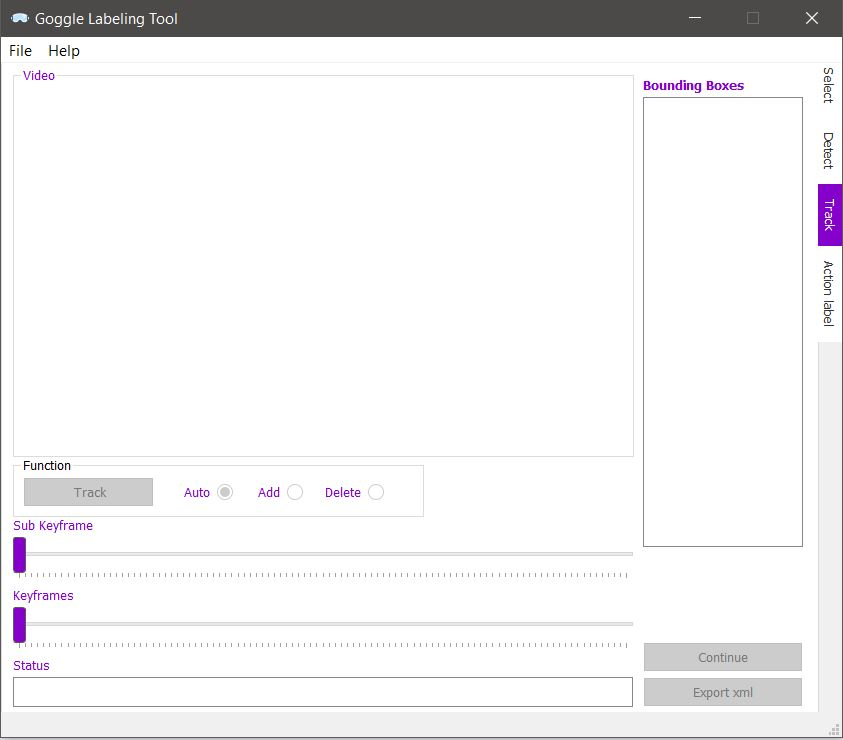
\includegraphics[scale=0.4]{chapter4/images/Final_ui/Track.jpg}
    \caption{รูปหน้าต่างแสดงผลของหน้าต่าง Track}
    \label{fig:final_track}
\end{figure}
จากรูปที่ \ref{fig:final_track} แสดงหน้าต่าง Track ของแอพพลิเคชั่น ซึ่งเมื่อเทียบกันกับฉบับร่างตามรูปที่ (\ref{fig:TrackDraft}) จะมีส่วนที่เพิ่มเติมขึ้นมาดังนี้
\begin{enumerate}
	\item ปรับหน้าตาโหมดการทำงานแบบอัตโนมัติและกำหนดเองจากฉบับร่างเพื่อให้สามารถใช้งานได้สะดวกขึ้น
	\item เพิ่มแถบเลื่อนเป็น 2 แถบเลื่อนทำให้สามารถดูคีย์เฟรมและเฟรมที่อยู่ระหว่างช่วงคีย์เฟรมได้สะดวกขึ้น
	\item เพิ่มปุ่มสำหรับนำผลลัพธ์ออกเป็นไฟล์ xml 
	\item แถบแสดงสถานะกระบวนการทำงาน
	\item แถบสำหรับคำแนะนำช่วยเหลือ
\end{enumerate}		

\clearpage
\subsection*{หน้าต่าง Label}
\begin{figure}[!ht]
  \centering
    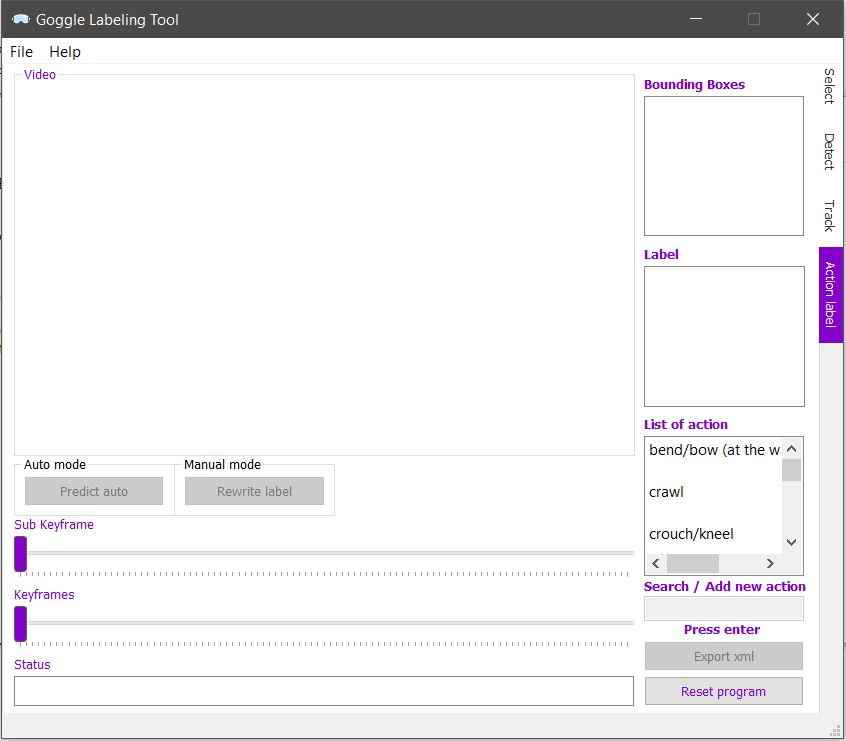
\includegraphics[scale=0.4]{chapter4/images/Final_ui/Label.jpg}
    \caption{รูปหน้าต่างแสดงผลของหน้าต่าง Label}
    \label{fig:final_label}
\end{figure}
จากรูปที่ \ref{fig:final_label} แสดงหน้าต่าง Label ของแอพพลิเคชั่น ซึ่งเมื่อเทียบกันกับฉบับร่างตามรูปที่ (\ref{fig:ActionLabelDraft}) จะมีส่วนที่เพิ่มเติมขึ้นมาดังนี้
\begin{enumerate}
	\item ปรับหน้าตาโหมดการทำงานแบบอัตโนมัติและกำหนดเองจากฉบับร่างเพื่อให้สามารถใช้งานได้สะดวกขึ้น
	\item เพิ่มแถบเลื่อนเป็น 2 แถบเลื่อนทำให้สามารถดูคีย์เฟรมและเฟรมที่อยู่ระหว่างช่วงคีย์เฟรมได้สะดวกขึ้น
	\item เครื่องมือสำหรับค้นหาหรือเพิ่มหมวดหมู่ของการกระทำ
	\item แถบแสดงสถานะกระบวนการทำงาน
	\item ปุ่มสำหรับเริ่มต้นการทำงานใหม่ 
	\item แถบสำหรับคำแนะนำช่วยเหลือ
\end{enumerate}		

\clearpage
\subsection{ผลลัพธ์การทำงานในแต่ละหน้าต่างของแอพพลิเคชั่น}
\subsection*{ผลลัพธ์การทำงานของหน้าต่าง Select}
\begin{figure}[!ht]
  \centering
    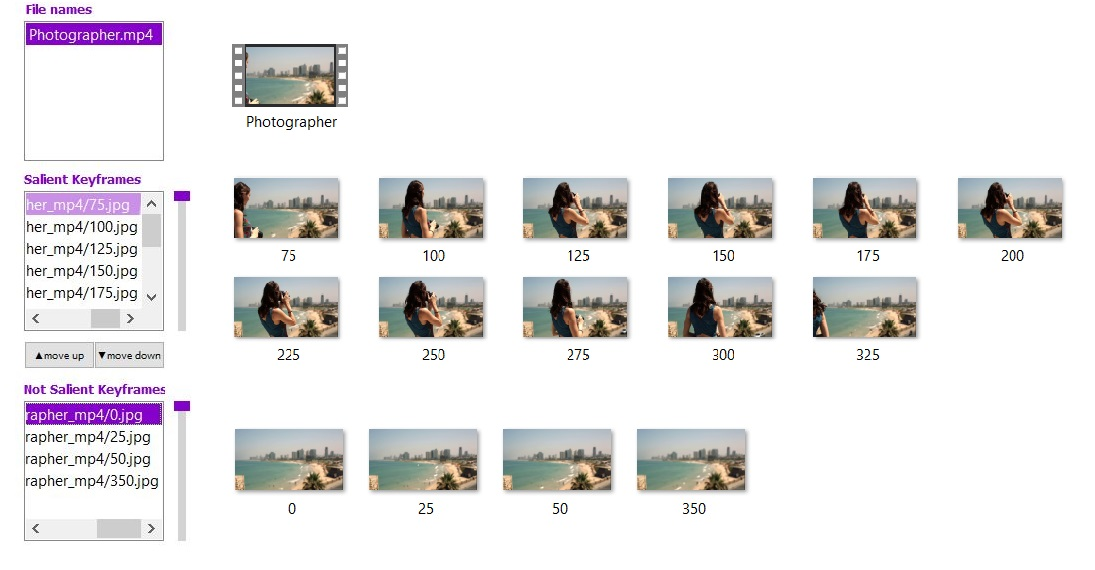
\includegraphics[scale=0.6]{chapter4/images/Result/result_select3.jpg}
    \caption{รูปผลลัพธ์การแยกเฟรมที่มีมนุษย์อยู่และไม่มีมนุษย์อยู่ภายในเฟรม}
    \label{fig:result_select}
\end{figure}
ขั้นตอนแรกแอพพลิเคชั่นจะสกัดแยกวิดิโอออกเป็นเฟรมทั้งหมด และทำการสุ่มคีย์เฟรมออกมาตามความถี่ที่ผู้ใช้ตั้งไว้ จากนั้นแอพพลิเคชั่นจะนำโมเดล YOLO-v3 320 
มาตรวจสอบว่าแต่ละคีย์เฟรมมีเฟรมใดบ้างที่มีมนุษย์อยู่ภายในเฟรม จากนั้นจะทำการแยกเฟรมที่มีมนุษย์อยู่และไม่มีมนุษย์อยู่ ดังรูปที่ \ref{fig:result_select}


\subsection*{ผลลัพธ์การทำงานของหน้าต่าง Detect}
\begin{figure}[!ht]
  \centering
    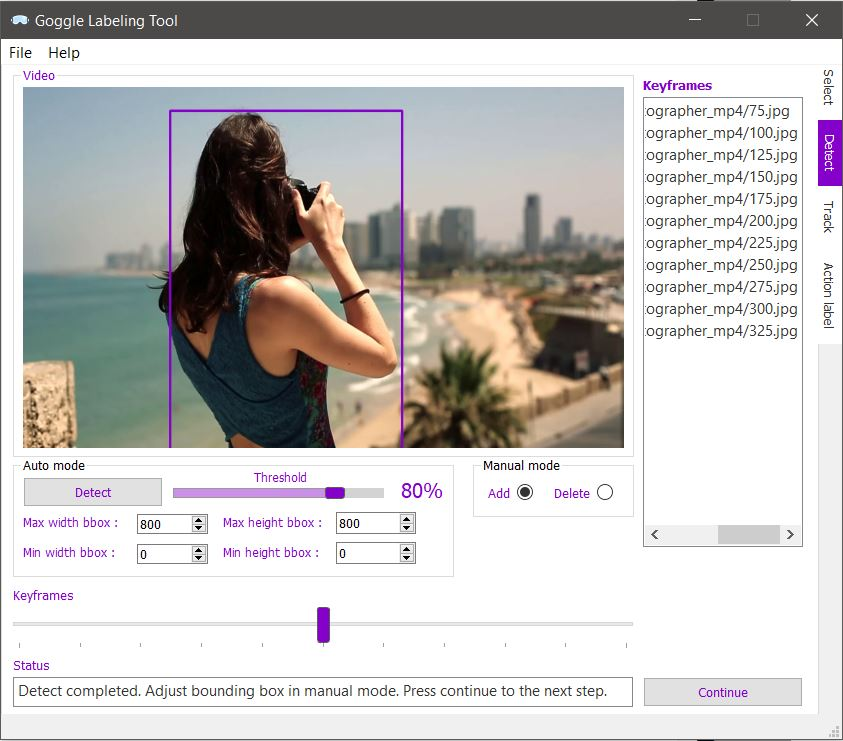
\includegraphics[scale=0.60]{chapter4/images/Result/result_select4.jpg}
    \caption{รูปคีย์เฟรมที่ถูกตีกรอบสี่เหลี่ยมในส่วนที่มีมนุษย์อยู่}
    \label{fig:result_detect}
\end{figure}
\clearpage
แอพพลิเคชั่นจะนำคีย์เฟรมที่มนุษย์ที่ได้จากหน้าต่าง Select นำมาตีกรอบสี่เหลี่ยมในส่วนของเฟรมที่มีมนุษย์อยู่โดยสามารถใช้โหมดการทำงานแบบอัตโนมัติหรือแบบแก้ไขเองก็ได้ 
ซึ่งผลลัพธ์ที่ได้จะได้คีย์เฟรมที่มีกรอบสี่เหลี่ยม ดังรูปที่ \ref{fig:result_detect} จากนั้นจะบันทึกข้อมูลในไฟล์ txt 

\subsection*{ผลลัพธ์การทำงานของหน้าต่าง Track}
\begin{figure}[!ht]
    \centering
   \begin{subfigure}[b]{0.4\linewidth}
      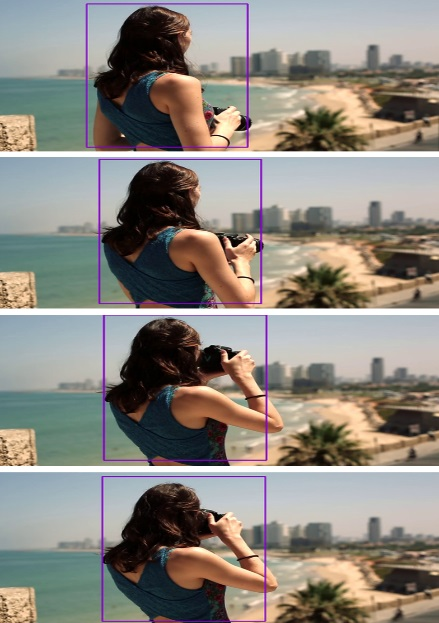
\includegraphics[width=\linewidth]{chapter4/images/Result/result_select6.jpg}
      \caption{ตัวอย่างเฟรมที่ถูกตีกรอบสี่เหลี่ยม}
      \label{fig:result_tracked}
    \end{subfigure}
\\
    \begin{subfigure}[b]{0.7\linewidth}
      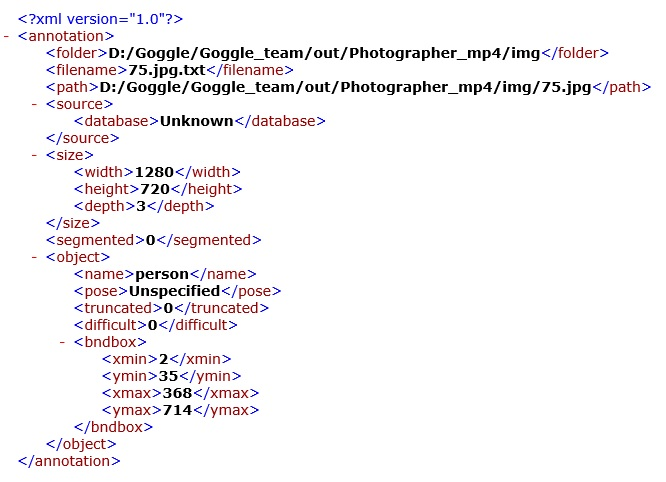
\includegraphics[width=\linewidth]{chapter4/images/Result/result_select7.jpg}
      \caption{ตัวอย่างไฟล์ xml}
      \label{fig:result_track_xml}
    \end{subfigure}
    \caption{รูปผลลัพธ์การทำงานของหน้าต่าง Track}
    \label{fig:result_track}
  \end{figure}
แอพพลิเคชั่นจะนำคีย์เฟรมที่ถูกตีกรอบสี่เหลี่ยมจากหน้าต่าง Detect มาทำนายกรอบสี่เหลี่ยมในเฟรมที่เหลือระหว่างช่วงคีย์เฟรม ซึ่งผลลัพธ์ที่ได้จะได้เฟรมทุกเฟรมที่มีมนุษย์อยู่จะถูกตีกรอบสี่เหลี่ยม 
ดังรูปที่ \ref{fig:result_tracked} จากนั้นสามารถบันทึกข้อมูลออกเป็นไฟล์ xml ได้ดังรูปที่ \ref{fig:result_track_xml}

\clearpage
\subsection*{ผลลัพธ์การทำงานของหน้าต่าง Label}
\begin{figure}[!ht]
    \centering
   \begin{subfigure}[b]{0.65\linewidth}
      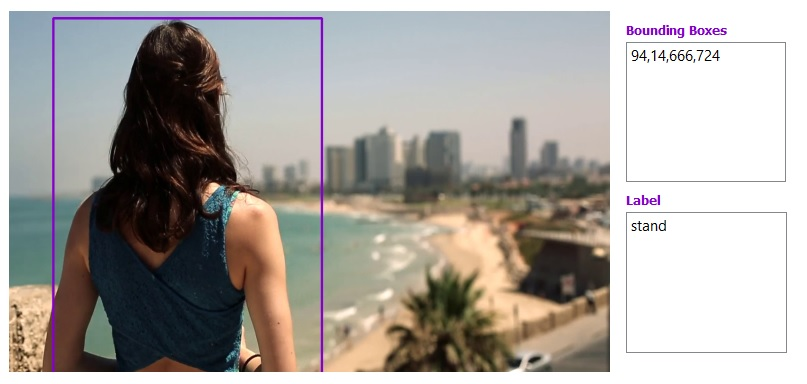
\includegraphics[width=\linewidth]{chapter4/images/Result/result_select.jpg}
      \caption{ตัวอย่างเฟรมที่ถูกตีกรอบสี่เหลี่ยมและคำทำนายการกระทำ}
      \label{fig:result_labeled}
    \end{subfigure}
\\
    \begin{subfigure}[b]{0.8\linewidth}
      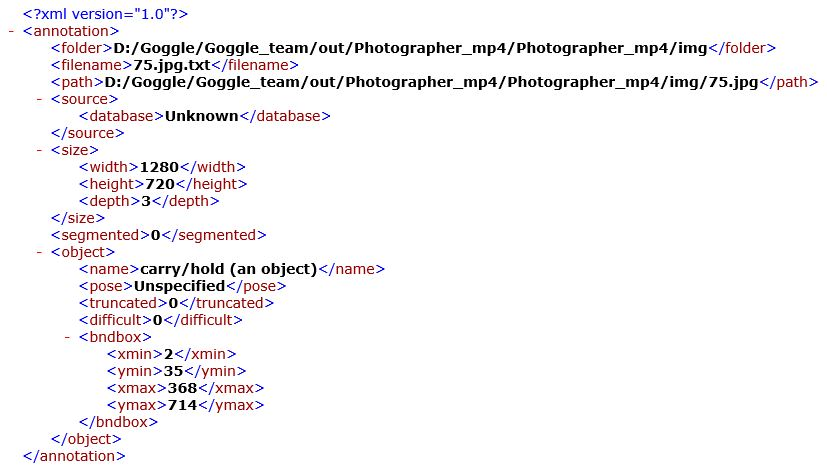
\includegraphics[width=\linewidth]{chapter4/images/Result/result_select9.jpg}
      \caption{ตัวอย่างไฟล์ xml}
      \label{fig:result_label_xml}
    \end{subfigure}
    \caption{รูปผลลัพธ์การทำงานของหน้าต่าง Label}
    \label{fig:result_label}
  \end{figure}
แอพพลิเคชั่นจะนำกรอบสี่เหลี่ยมของทุกเฟรมที่มีมนุษย์อยู่มาทำนายมนุษย์ในกรอบสี่เหลี่ยมนั้นกำลังมีการกระทำอะไรอยู่ โดยสามารถทำงานได้ทั้งโหมดอัตโนมัติหรือแบบแก้ไขเอง 
และสามารถบันทึกข้อมูลออกเป็นไฟล์ xml ได้ดังรูปที่ \ref{fig:result_label_xml}
